\setcounter{page}{56} % начать нумерацию страниц с 56
\newpage
\setlength{\columnsep}{1cm} % расстояние между столбцами текста
\begin{multicols}{2} % разделить структуру страницы на две колонки
\fancyhf{}
\chead{\footnotesize
О Т В Е Т Ы , У К А З А Н И Я , Р Е Ш Е Н И Я}
\rhead{\thepage}
\begin{wrapfigure}{l}{0.5\linewidth}
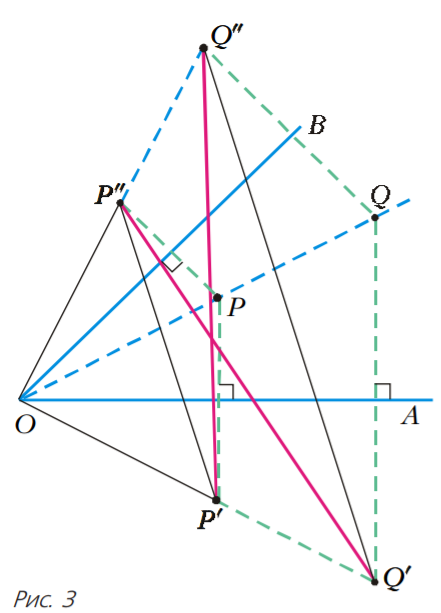
\includegraphics[scale=0.5]{img1.png}
\end{wrapfigure}
    \noindent
    Обратим внимание, что по условию первыми «стреляли» бактерии, причем произвели они не менее \emph{двух} «залпов». Так что рассмотренный сейчас момент (когда имеется 9\emph{М} бактерий и 31\emph{М} вирусов) вполне мог бы быть исходным. В этом случае общее количество микробов равно 9\emph{М} + 31\emph{М} = 40\emph{М}, а так как по условию это число равно 2000, то \emph{М} = 2000/40 = 50. Таким образом, в данном случае в итоге борьбы осталось в живых 50 бактерий и 50 вирусов. Предположение, что этот обмен любезностями продолжался дольше, приводит к противоречию. Рассмотрев аналогично вторую возможность, когда последний удар нанесли вирусы, опять получаем противоречие с условием. \\ 
    Итак, ответ: в результате разразившегося побоища в живых осталось по 50 бактерий и вирусов.
    \begin{center}
        \large
        \emph{Задачи}\\
    \end{center}
    \begin{center}
        \emph{(см. «Квант» №5)}
    \end{center}
    \textbf{1.} Слагаемых ШАХ меньше 10, иначе их сумма была бы четырехзначной. Запишем ребус в виде $ШАХ \times У = МАТ$, где У – неизвестная отличная от 0 цифра, возможно совпадающая с одной из цифр, зашифрованных буквами Ш, А, Х, М, Т. Цифры Ш = 1, А = 3, Х = 4, М = 9, Т = 8 удовлетворяют ребусу: $134 \times 7 = 938$. Покажем, что значение У = 7 наибольшее. \\ 
    Предположим, что У = 8 или У = 9. Поскольку в этом случае наименьшим трехзначным числом, представленным словом ШАХ, является число 123 (так как $Ш = 1, А \neq 0, Х \neq 0$), то значение У = 9 не подходит: $123 \times 9 = 1107$. Легко проверить, что в случае У = 8 и наименьшем значении А = 2 ребус $12Х \times 8 = 92Т$ для букв Х и Т решений не имеет, в случае же $А \geq 3$ произведение $1АХ \times 8$ получается четырехзначным. Итак, гроссмейстер объявил шах семь раз. \\ 
    \textbf{2.} Пусть первая программа содержала \emph{K} клипов. Тогда, по условию, вторая программа содержала 1,5\emph{K} клипов, а Бивису понравились \emph{K}/5 клипов первой программы и (1,5\emph{K}) : 2 = 3\emph{K}/4 клипов второй программы. По смыслу задачи все эти числа должны быть целыми, откуда следует, что \emph{K} делится на 4 и на 5, т.е. на 20. Итак, \emph{K} = 20\emph{m}, где \emph{m} – натуральное число. Тогда вторая программа содержала $1,5 \times 20m = 30m$ клипов, а третья программа – все остальные, т.е. $200 - 20m - 30m = 200 - 50m$ клипов. Это число должно быть положительным, в связи с чем $200 - 50m > 0$, откуда $m < 4$. Далее, Бивису понравились всего  $(20m/5) + (30m/2) = 19m$ клипов. Батт-Хеду понравилось столько же клипов, причем в это число входили все клипы третьей программы. Поэтому $19m \geq 200 - 50m$, и $m \geq 200/69 > 2,8$.\\ 
    Таким образом, $2,8 < m < 4$. Единственное натуральное число, удовлетворяющее этим условиям, это \emph{m} = 3. Этот результат позволяет нам восстановить всю картину. Итак, первая программа содержала $20 \times 3 = 60$ клипов, вторая – $1,5 \times 60 =  90$ клипов, третья $200 - 60 - 90 = 50$ клипов. Бивису понравились $(60/5) + (90/2) = 57$ клипов, Батт-Хеду – столько же. Ну, а не понравилось каждому из них $200 - 57 = 143$ клипа. \\ 
    \textbf{3.} Сомкнем выходящие из города дороги в еще один перекресток. Пусть \emph{N} – общее количество перекрестков вместе с этим. Так как в каждом из перекрестков сходится по три дороги, то общее количество оконечностей дорог 3\emph{N}. Это число четное, поскольку каждая дорога в нашем случае имеет два конца. Следовательно, число \emph{N} – четное, и в городе имеется нечетное количество перекрестков. Поскольку в каждом из них сходятся по одной дороге трех разных цветов, то для каждого цвета найдется дорога, не имеющая двух оконечностей в городе. Итак, все три выходящие из города дороги непременно имеют разные цвета.\\ 
    \textbf{4.} Воспользуемся следующим очевидным утверждением. Имеется \emph{K} карточек. Известно, что какие бы \emph{M} из них ни взять, среди них окажется не менее \emph{N} особых. В этом случае среди \emph{K} карточек имеется не менее $K - M + N$ особых. Считая, что особые карточки – синие, в приложении к условию задачи имеем:\\
    \begin{center}
        \begin{tabular}{|c|c|c|c|}
            \hline
            \emph{K} & \emph{M} & \emph{N} & \emph{K - M + N} \\ \hline
            100 & 80 & 20 & 40 \\ \hline
            40 & 10 & 2 & 32 \\ 
            \hline
        \end{tabular}
    \end{center}
    Считая, что особые карточки – красные, в приложении к условию задачи имеем: \\
    \begin{center}
        \begin{tabular}{|c|c|c|c|}
            \hline
            \emph{K} & \emph{M} & \emph{N} & \emph{K - M + N} \\ 
            \hline
            100 & 50 & 30 & 80 \\ \hline
            80 & 20 & 10 & 70 \\ \hline
            70 & 5 & 3 & 68 \\ 
            \hline
        \end{tabular}
    \end{center}
    Итак, в колоде находятся 32 синих и 68 красных карточек.\\ 
    \textbf{5.} Нет, не удастся. Если бы существовало разбиение пятиугольного поля на параллелограммы, то можно было бы пройти от любого края поля к другому краю, двигаясь по цепочке параллелограммов. Поскольку в пятиугольнике не для каждой стороны существует параллельная ей сторона, то этого сделать нельзя.
    \begin{center}
        \textbf{Кеплер и винные бочки – австрийские и рейнские}
    \end{center}
    \textbf{1.} Учитывая, что AB = OA/\emph{sin a}, имеем \[E = \frac{C}{OA^2} \sin^2 \alpha \cos^2 \alpha . \]  Таким образом, если лампу поместить в вершину конуса максимального объема, то окружность его основания получит наибольшую освещенность.\\  
    \textbf{2.} Обозначим $a = 4 - x$, тогда $b = 4 + x$ и $ab(b - a) = ax(16 - x^2)$, причем $0\leq x \leq 4$. Максимум достигается при $x = 4/\sqrt{3}$ и равен $256/(3\sqrt{3})$. \\ 
    \textbf{3.} Обозначим буквой \emph{R} радиус шара, а буквами \emph{r} и \emph{h} – радиус и высоту конуса. Тогда объем конуса равен $V = \pi r^2h/3$.Продолжив высоту конуса до пересечения с шаром, получим отрезок длиной $2R - h$. Таким образом, через одну точку (центр основания конуса) проходят две хорды: одна из них состоит из отрезков длиной \emph{h} и $2R - h$, а другая – из двух отрезков длиной \emph{r} каждый. Значит, $r^2 = h(2R - h)$, так что $V = \pi h^2(2R - h)/3$. Применяя неравенство о среднем арифметическом и среднем геометрическом, получим \[\frac{3V}{4\pi} = \frac{h}{2}\cdot\frac{h}{2}\cdot(2R - h)\leq\left(\frac{\dfrac{h}{2} + \dfrac{h}{2} + 2R - h}{3}\right)^3 = \frac{8}{27}R^3,\] где равенство достигается при $\dfrac{h}{2} = 2R - h$, т.е. при $h = \dfrac{4}{3}R$.
\end{multicols}